\documentclass[tikz,border=2pt,png]{standalone}
\usepackage{tkz-euclide}
\usetkzobj{all}

\begin{document}
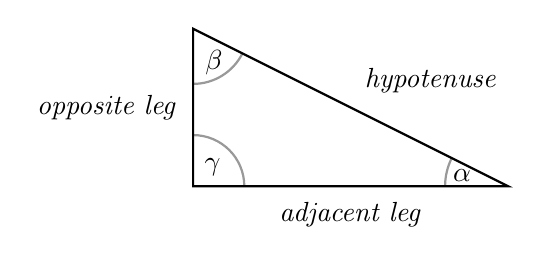
\begin{tikzpicture}[thick]
\coordinate (O) at (0,0);
\coordinate (A) at (4,0);
\coordinate (B) at (0,2);
\draw (O)--(A)--(B)--cycle;

\tkzLabelSegment[below=2pt](O,A){\textit{adjacent leg}}
\tkzLabelSegment[left=2pt](O,B){\textit{opposite leg}}
\tkzLabelSegment[above right=2pt](A,B){\textit{hypotenuse}}

\tkzMarkAngle[fill= orange,size=0.65cm,%
opacity=.4](A,O,B)
\tkzLabelAngle[pos = 0.35](A,O,B){$\gamma$}

\tkzMarkAngle[fill= orange,size=0.8cm,%
opacity=.4](B,A,O)
\tkzLabelAngle[pos = 0.6](B,A,O){$\alpha$}

\tkzMarkAngle[fill= orange,size=0.7cm,%
opacity=.4](O,B,A)
\tkzLabelAngle[pos = 0.5](O,B,A){$\beta$}


\end{tikzpicture}
\end{document}